\section{TASK 4, Testing the networks}

\begin{frame}
	\frametitle{Euler's method -- linear system}
	\paragraph{Dataset}\vspace{-2mm}
	\begin{itemize}
		\item 1 Mio. random samples of $\overrightarrow{x}_{n}$ and $\overrightarrow{x}_{n+1}$
		\item Samples between $-100$ and $100$ (both $x_1$ and $x_2$)
	\end{itemize}
	\paragraph{Trajectories}\vspace{-2mm}
	\begin{figure}[H]
		\subfloat[$x_0 = (100, -100)$]{
			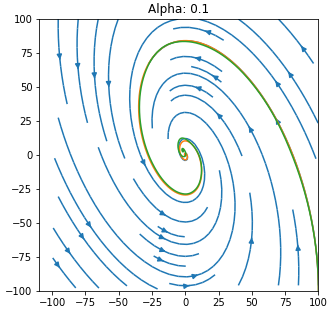
\includegraphics[width=.30\linewidth]{figures/euler/ls_100_-100.png}
		}\quad
		\subfloat[$x_0 = (-75, 100)$]{
			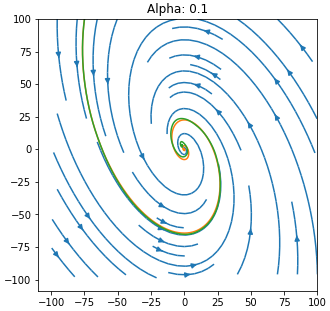
\includegraphics[width=.30\linewidth]{figures/euler/ls_-75_100.png}
		}\quad
		\subfloat[$x_0 = (-100, 25)$]{
			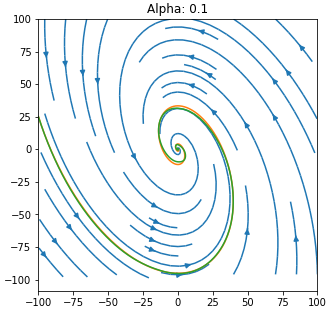
\includegraphics[width=.30\linewidth]{figures/euler/ls_-100_25.png}
		}
		\caption{Phase diagrams for different values of $x_0$.}
	\end{figure}
\end{frame}

\begin{frame}
	\frametitle{Euler's method -- Andronov-Hopf system}
	\paragraph{Dataset}\vspace{-2mm}
	\begin{itemize}
		\item 1000 trajectories
		\item Trajectories starting between $-5$ and $5$ (both $x_1$ and $x_2$)
		\item $alpha$ values between $-3$ and $3$
	\end{itemize}
	\paragraph{Trajectories}\vspace{-2mm}
	\begin{figure}[H]
		\subfloat[$x_0 = (2, -2)$; $alpha = -1$]{
			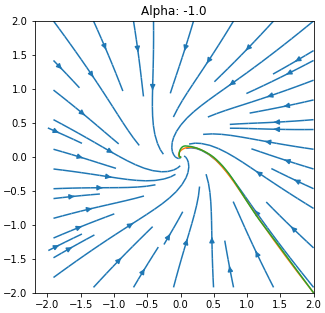
\includegraphics[width=.30\linewidth]{figures/euler/and_hopf_a_-1.png}
		}\quad
		\subfloat[$x_0 = (2, -2)$; $alpha = 0$]{
			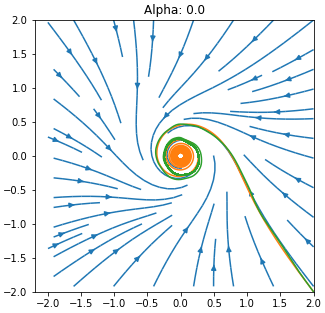
\includegraphics[width=.30\linewidth]{figures/euler/and_hopf_a_0.png}
		}\quad
		\subfloat[$x_0 = (2, -1)$; $alpha = 1$]{
			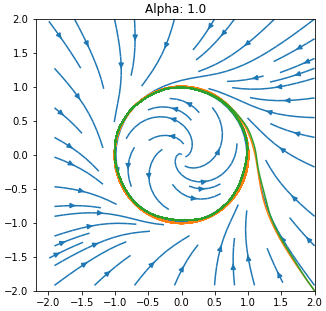
\includegraphics[width=.30\linewidth]{figures/euler/and_hopf_a_1.png}
		}
		\caption{Phase diagrams for different values of $alpha$.}
	\end{figure}
\end{frame}

\begin{frame}
	\frametitle{Euler's method -- R\"ossler attractor}
	\paragraph{Dataset}\vspace{-2mm}
	\begin{itemize}
		\item 150 trajectories
		\item Trajectories starting between $0$ and $10$ (for $x_1$, $x_2$ and $x_3$)
		\item $a$ values between $-0.1$ and $0.3$
	\end{itemize}
	\paragraph{Trajectories}\vspace{-2mm}
	\begin{figure}[H]
		\subfloat[$x_0 = (5, 5, 5)$; $a = -0.1$]{
			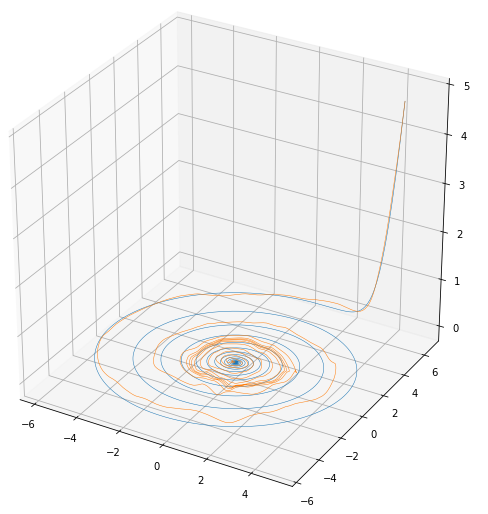
\includegraphics[width=.35\linewidth]{figures/euler/roe_-0_1.png}
		}\quad
		\subfloat[$x_0 = (5, 5, 5)$; $a = 0.0$]{
			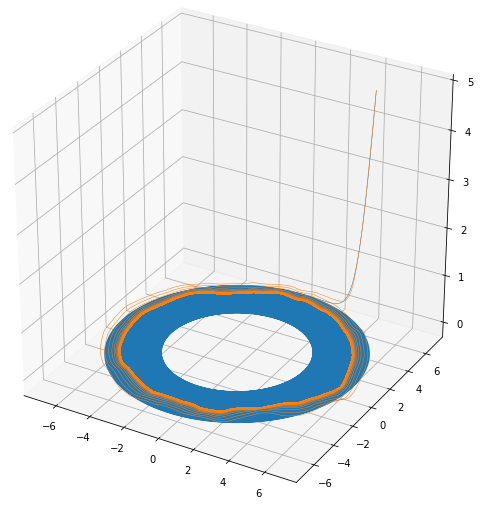
\includegraphics[width=.35\linewidth]{figures/euler/roe_0_0.png}
		}
		\caption{Phase diagrams for different values of $a$.}
	\end{figure}
\end{frame}

\begin{frame}
	\frametitle{Euler's method -- R\"ossler attractor}
	\paragraph{Trajectories}\vspace{-1mm}
	\begin{figure}[H]
		\subfloat[$x_0 = (5, 5, 5)$; $a = 0.1$]{
			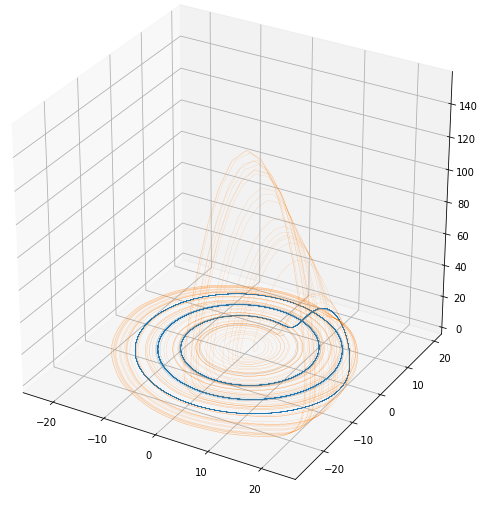
\includegraphics[width=.30\linewidth]{figures/euler/roe_0_1.png}
		}\quad
		\subfloat[$x_0 = (5, 5, 5)$; $a = 0.2$]{
			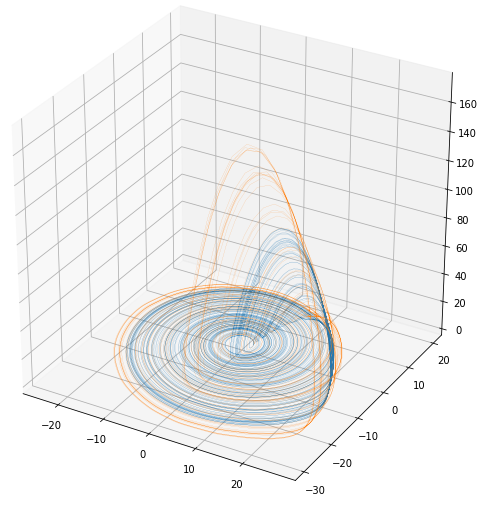
\includegraphics[width=.30\linewidth]{figures/euler/roe_0_2.png}
		}\quad
		\subfloat[$x_0 = (5, 5, 5)$; $a = 0.3$]{
			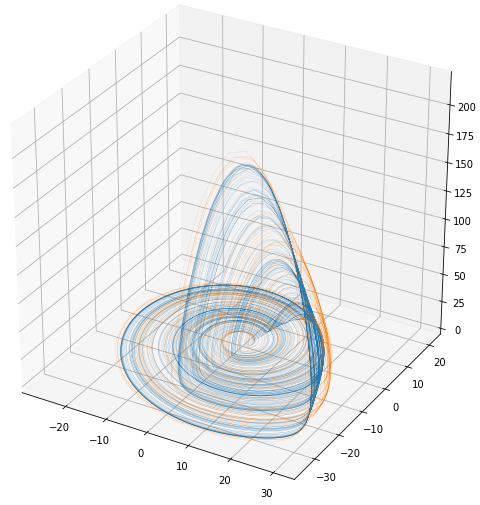
\includegraphics[width=.30\linewidth]{figures/euler/roe_0_3.png}
		}
		\caption{Phase diagrams for different values of $a$.}
	\end{figure}
\end{frame}

\begin{frame}
	\frametitle{Runge-Kutta method -- linear system}
	\paragraph{Dataset}\vspace{-2mm}
	\begin{itemize}
		\item 1 Mio. random samples of $\overrightarrow{x}_{n}$ and $\overrightarrow{x}_{n+1}$
		\item Samples between $-100$ and $100$ (both $x_1$ and $x_2$)
	\end{itemize}
	\paragraph{Trajectories}\vspace{-2mm}
	\begin{figure}[H]
		\subfloat[$x_0 = (100, -100)$]{
			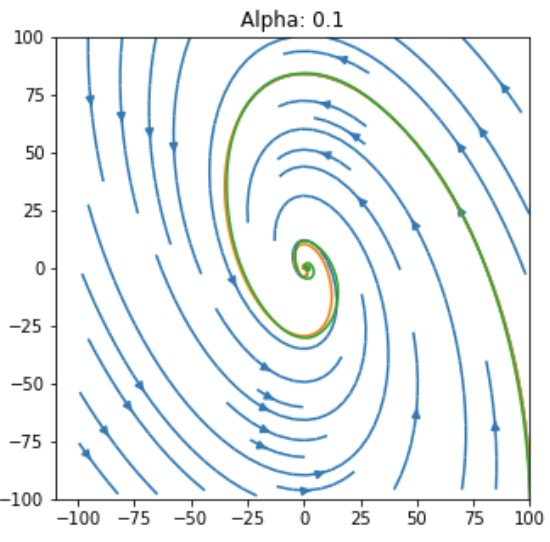
\includegraphics[width=.30\linewidth]{figures/runge_kutta/ls_100_-100.png}
		}\quad
		\subfloat[$x_0 = (-75, 100)$]{
			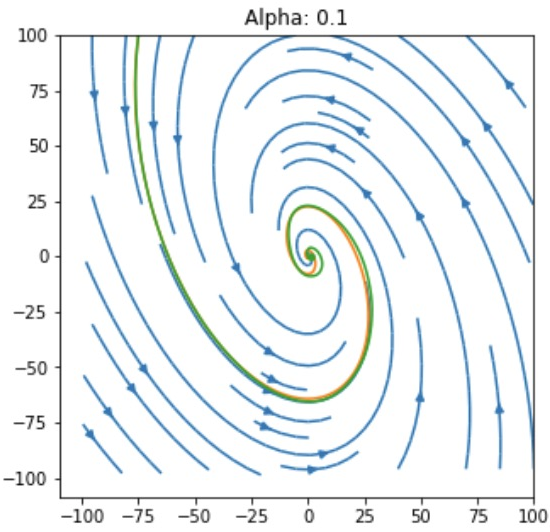
\includegraphics[width=.30\linewidth]{figures/runge_kutta/ls_-75_100.png}
		}\quad
		\subfloat[$x_0 = (-100, 25)$]{
			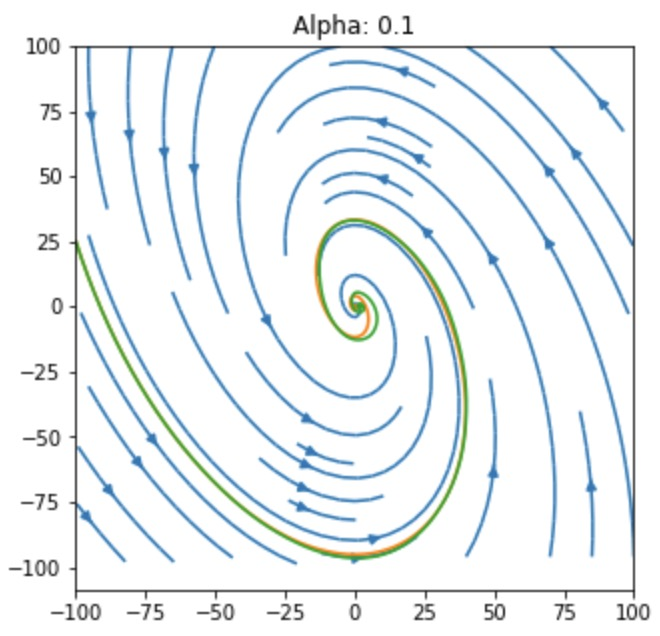
\includegraphics[width=.30\linewidth]{figures/runge_kutta/ls_-100_25.png}
		}
		\caption{Phase diagrams for different values of $x_0$.}
	\end{figure}
\end{frame}

\begin{frame}
	\frametitle{Runge-Kutta method -- Andronov-Hopf system}
	\paragraph{Dataset}\vspace{-2mm}
	\begin{itemize}
		\item 1000 trajectories
		\item Trajectories starting between $-5$ and $5$ (both $x_1$ and $x_2$)
	\end{itemize}
	\paragraph{Trajectories}\vspace{-2mm}
	\begin{figure}[H]
		\subfloat[$x_0 = (2, -2)$; $alpha = -1$]{
			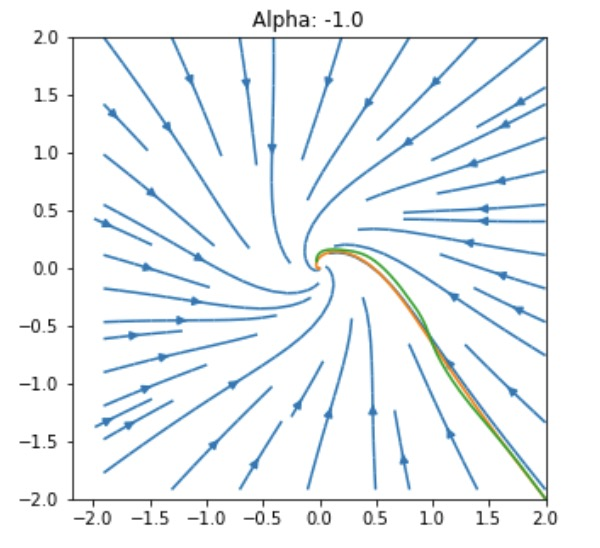
\includegraphics[width=.30\linewidth]{figures/runge_kutta/and_hopf_a_-1.png}
		}\quad
		\subfloat[$x_0 = (2, -2)$; $alpha = 0$]{
			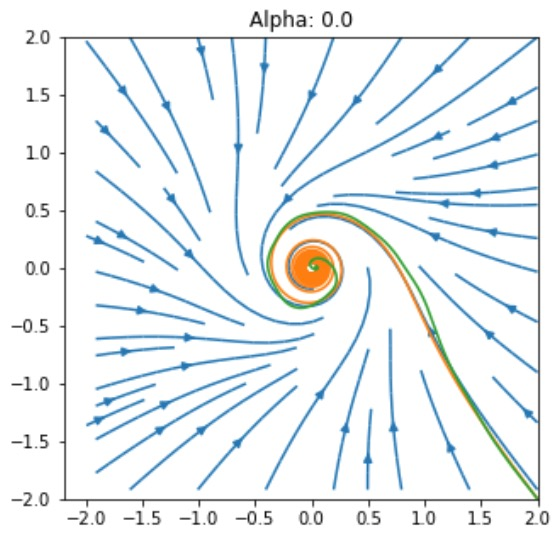
\includegraphics[width=.30\linewidth]{figures/runge_kutta/and_hopf_a_0.png}
		}\quad
		\subfloat[$x_0 = (2, -2)$; $alpha = 1$]{
			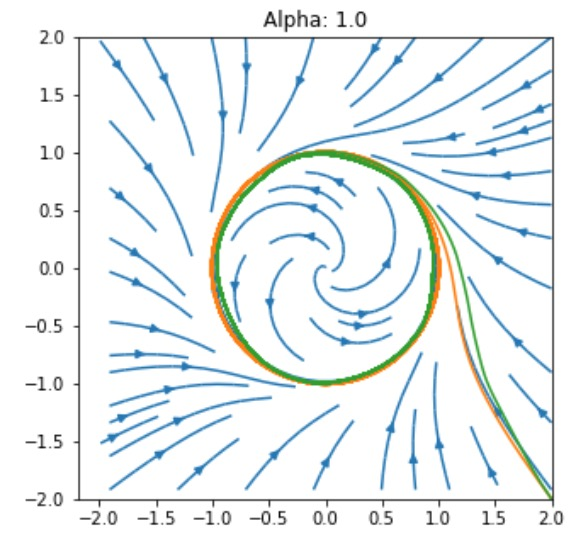
\includegraphics[width=.30\linewidth]{figures/runge_kutta/and_hopf_a_1.png}
		}
		\caption{Phase diagrams for different values of $alpha$.}
	\end{figure}
\end{frame}

\begin{frame}
	\frametitle{Runge-Kutta method -- R\"ossler attractor}
	\paragraph{Dataset}\vspace{-2mm}
	\begin{itemize}
		\item 150 trajectories
		\item Trajectories starting between $0$ and $10$ (for $x_1$, $x_2$ and $x_3$)
		\item $a$ values between $-0.1$ and $0.3$
	\end{itemize}
	\paragraph{Trajectories}\vspace{-2mm}
	\begin{figure}[H]
		\subfloat[$x_0 = (5, 5, 5)$; $a = -0.1$]{
			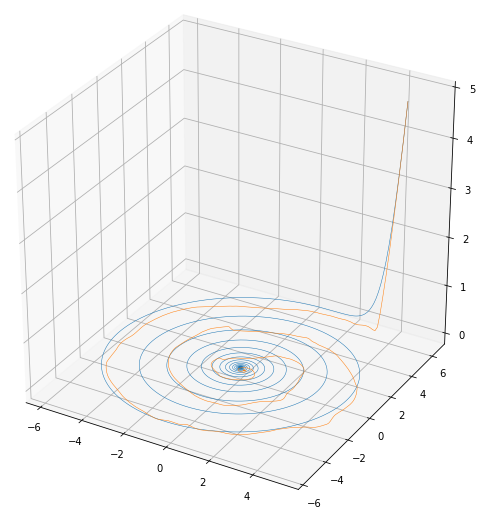
\includegraphics[width=.35\linewidth]{figures/runge_kutta/roe_-0_1.png}
		}\quad
		\subfloat[$x_0 = (5, 5, 5)$; $a = 0.0$]{
			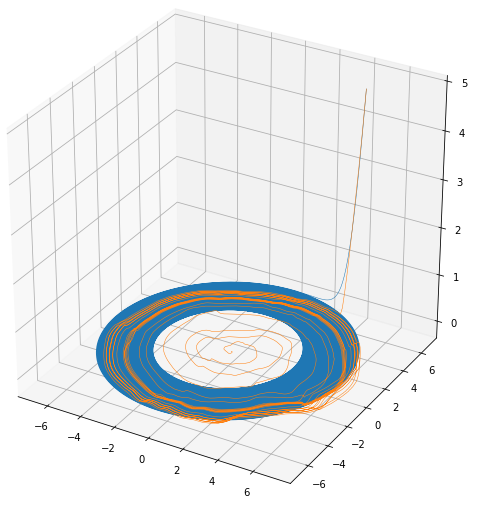
\includegraphics[width=.35\linewidth]{figures/runge_kutta/roe_0_0.png}
		}
		\caption{Phase diagrams for different values of $a$.}
	\end{figure}
\end{frame}

\begin{frame}
	\frametitle{Runge-Kutta method -- R\"ossler attractor}
	\paragraph{Trajectories}\vspace{-1mm}
	\begin{figure}[H]
		\subfloat[$x_0 = (5, 5, 5)$; $a = 0.1$]{
			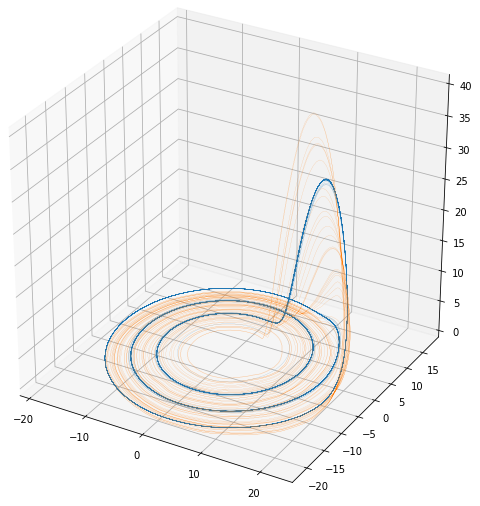
\includegraphics[width=.30\linewidth]{figures/runge_kutta/roe_0_1.png}
		}\quad
		\subfloat[$x_0 = (5, 5, 5)$; $a = 0.2$]{
			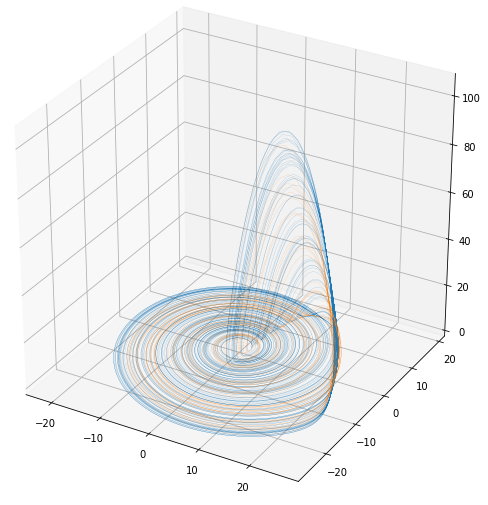
\includegraphics[width=.30\linewidth]{figures/runge_kutta/roe_0_2.png}
		}\quad
		\subfloat[$x_0 = (5, 5, 5)$; $a = 0.3$]{
			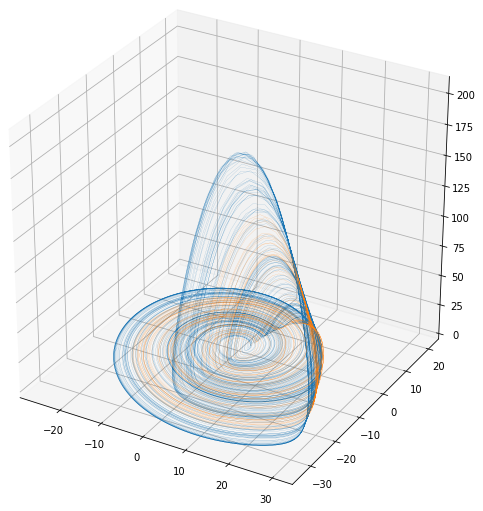
\includegraphics[width=.30\linewidth]{figures/runge_kutta/roe_0_3.png}
		}
		\caption{Phase diagrams for different values of $a$.}
	\end{figure}
\end{frame}
